\documentclass{article}
\usepackage{amsmath}
%\usepackage{subfigure}
\usepackage{subfig}
\usepackage{amsthm}
\usepackage{amssymb}
\usepackage{graphicx}
\usepackage{mdwlist}
\usepackage[colorlinks=true]{hyperref}
\usepackage{geometry}
\usepackage{titlesec}
\geometry{margin=1in}
\geometry{headheight=2in}
\geometry{top=2in}
\usepackage{palatino}
% \usepackage{mathrsfs}
\usepackage{fancyhdr}
\usepackage{paralist}
% \usepackage{todonotes}
\setlength{\marginparwidth}{2.15cm}
\usepackage{tikz}
\usetikzlibrary{positioning,shapes,backgrounds}
\usepackage{float} % Place figures where you ACTUALLY want it
\usepackage{comment}
\usepackage{ifthen}
\usepackage{biblatex}
\usepackage{courier}
\rhead{}
\lhead{}

\renewcommand{\baselinestretch}{1.15}

% Shortcuts for commonly used operators
\newcommand{\E}{\mathbb{E}}
\newcommand{\Var}{\operatorname{Var}}
\newcommand{\Cov}{\operatorname{Cov}}
\DeclareMathOperator{\argmin}{arg\,min}
\DeclareMathOperator{\argmax}{arg\,max}

% do not number subsection and below
\setcounter{secnumdepth}{1}

% custom format subsection
\titleformat*{\subsection}{\large\bfseries}

% set up the \question shortcut
\newcounter{question}[section]
\newenvironment{question}[1][]
  {\refstepcounter{question}\par\addvspace{1em}\textbf{Question~\Alph{question}\!
    \ifthenelse{\equal{#1}{}}{}{ [#1 points]}: }}
    {\par\vspace{\baselineskip}}

\newcounter{subquestion}[question]
\newenvironment{subquestion}[1][]
  {\refstepcounter{subquestion}\par\medskip\textbf{\roman{subquestion}.\!
    \ifthenelse{\equal{#1}{}}{}{ [#1 points]:}} }
  {\par\addvspace{\baselineskip}}

\titlespacing\section{0pt}{12pt plus 2pt minus 2pt}{0pt plus 2pt minus 2pt}
\titlespacing\subsection{0pt}{12pt plus 4pt minus 2pt}{0pt plus 2pt minus 2pt}
\titlespacing\subsubsection{0pt}{12pt plus 4pt minus 2pt}{0pt plus 2pt minus 2pt}



\chead{%
  {\vbox{%
      \vspace{2mm}
      \large
      Networks: Structure \& Economics \hfill
      Caltech CMS/CS/EE 144 \hfill \\[1pt]
      Miniproject 1\hfill
      February $8^{\text{rd}}$, 2016 \\
    }
  }
}

\begin{document}
\pagestyle{fancy}

\LARGE
\begin{center}
\textbf{Churn}

\large
John Li, Albert Ge, Timothy Chou, Kevin Chang

Rankmaniac Report

\end{center}

\normalsize
\medskip

\section{Overview}
During this Pandemaniac project, our group ``churn'' implemented a number of algorithms to choose 
seed nodes in a network to optimize the spread of a simulated epidemic across the graph. 
The code was written in a Python base. 

\subsection*{Counterexample}
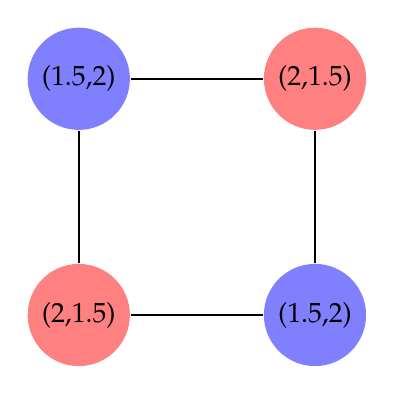
\begin{tikzpicture}[auto,node distance=3cm, thick,main node/.style={circle,fill=blue!50,minimum size=1cm},sub node/.style={circle,fill=red!50,minimum size=1cm}]
\node[main node] (1) {(1.5,2)};
\node[sub node] (2) [right of=1] {(2,1.5)};
\node[sub node] (3) [below of=1] {(2,1.5)};
\node[main node] (4) [right of=3] {(1.5,2)};

\path[draw, thick]
(1) edge node {} (2)
edge node {} (3)
(4) edge node {} (2)
edge node {} (3)
;
\end{tikzpicture}\\
Next iteration is\\
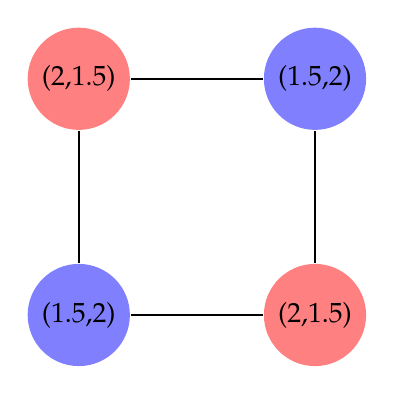
\begin{tikzpicture}[auto,node distance=3cm, thick,main node/.style={circle,fill=blue!50,minimum size=1cm},sub node/.style={circle,fill=red!50,minimum size=1cm}]
\node[sub node] (1) {(2,1.5)};
\node[main node] (2) [right of=1] {(1.5,2)};
\node[main node] (3) [below of=1] {(1.5,2)};
\node[sub node] (4) [right of=3] {(2,1.5)};

\path[draw, thick]
(1) edge node {} (2)
edge node {} (3)
(4) edge node {} (2)
edge node {} (3)
;
\end{tikzpicture}\\
Which we see cycles back to \\
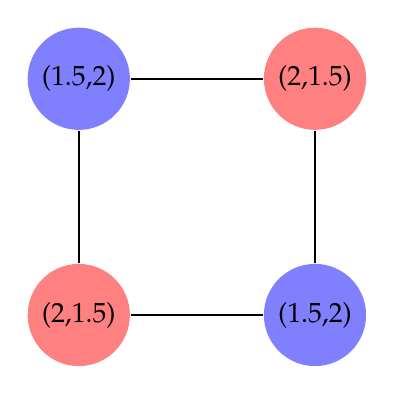
\begin{tikzpicture}[auto,node distance=3cm, thick,main node/.style={circle,fill=blue!50,minimum size=1cm},sub node/.style={circle,fill=red!50,minimum size=1cm}]
\node[main node] (1) {(1.5,2)};
\node[sub node] (2) [right of=1] {(2,1.5)};
\node[sub node] (3) [below of=1] {(2,1.5)};
\node[main node] (4) [right of=3] {(1.5,2)};

\path[draw, thick]
(1) edge node {} (2)
edge node {} (3)
(4) edge node {} (2)
edge node {} (3)
;
\end{tikzpicture}\\
Meaning equilibrium will never be reached. 
\section{Initial Framework}
    We began this project by first understanding and processing the data from the format of a JSON file.
    We wrote some initial files to load the data from a JSON file, and use some naive algorithm to
    pick seed nodes (described below).
    To present it in a file suitable for submission, a file \texttt{submit.py} was 
    created, which took in as its parameter the graph input file, and output results in a file
    \texttt{submit.txt} for upload.
    
    \subsection*{Early Bird Points} 
    To obtain early bird points, we first wrote a short file \texttt{deg\_centrality.py} which
    ranks the top X nodes by their degree value. Here X refers to the number of seeds
    to be picked, as denoted by the name of each graph JSON file. 
    
    \subsection*{Beating TA\_fewer and TA\_degree}
    The next algorithm we tried was tailored specifically to beat TA\_degree
    written in \texttt{deg\_centrality2.py}. Given that
    TA\_degree follows the exact same strategy, then all of the initial seed pickings
    would be cancelled by TA\_degree. To combat this, we would pick the top X-1 seeds by degree,
    and the last seed to just be a neighbor of the highest-degree node. The intuition 
    behind this is that, as the top X-1 nodes would be cancelled out, TA\_degree would be 
    left with the Xth-highest degree node, and we would have a neighbor to the 
    highest degree node. Thus, after a single step in a round, we would (ideally) obtain
    control of the highest degree node. 
    \\
    This algorithm ended up beating both TA\_fewer and TA\_degree, securing the remaining
    required points for the programming side of the project. 
     

\section{Development and Improvements}

\subsection*{Linear Combinations}

\subsection*{Top-K Mix}
This algorithm involved finding the degree centrality. closeness centrality, and betweeness centrality, then selecting the top $A, B, C$ respectively from each. 

\subsection*{Monte Carlo}
Monte Carlo simulations were done on the various linear combinations and top-K mixes. A number of samples of different linear combinations in .05 steps and every possible selection of A, B, C for a top-K mix was used to represent different strategies we were considering generating different seeds on 16 graphs. In addition, we also hand selected seeds in an attempt to immitate TA\_more. We then pitted all the strategies against each other, with one side getting the normal amount of seeds and the player 2 getting 20\% more seeds. Doing so involved playing approximately 2 million games, so the simulation was run (\texttt{runSim.py}) across multiple computers before the outputs were agreggated using \texttt{combineResults.py}. These results were then used for our final attempt against TA\_more. The final result was a linear combination with weights $[.70, .25, .5]$ which had won at least 5 out of 16 graphs against every player 2 (which had 20\% more seed nodes). 

\subsection*{Bridges}

\subsection*{Mixed Strategy}
    Using a mixed strategy requires some notion picking seed nodes according to some
    probability distribution. Each strategy will output 
    the rankings of the top X nodes, according to some centrality measure, 
    which provides a quantitative notion of how important a particular seed is relative 
    to others. Thus, our idea was to use the values of centrality measure as a rough
    probability of how likely it is to be selected as a node - the greater the measure,
    the more likely it is to be picked. This follows similarly with the idea of computing
    the probabilities of a mixed strategy - a particular action receives greater 
    probability if its expected payoff is greater. 
    \\
    In a file, \texttt{mixed.py}, we outline the procedure for computing a mixed strategy.
    Assuming that all centrality measures are equally important, we pick one of the
    measures at random, obtain a list of most important nodes according to that measure,
    and perform a weighted random choice among those nodes.
    \\
    \textbf{Results:} Using a mixed strategy for the bridge centrality measure,
    and degree centrality, we obtained a score of 2 on day3 of 
    the tournament. Though it wasn't much,
    this was the most points we've scored out of all three days of the tournament,
    and it seemed to be a promising avenue to explore given more time.
    
\section{Testing}
    We tested the algorithms for computing seed nodes by running them against
    each other, using the provided \texttt{sim.py}. To facilitate this,
    a wrapper class \texttt{runStrat.py} was created, which takes as arguments
    a variable number of strategies and a graph input, picks the seeds according to each strategy,
    and runs the simulation with seeds on the graph.



 % Can talk about data mining. What scripts we used. etc.
 

\section{Contributions}
There are four members in this group: Kevin Chang, Timothy Chou, Albert Ge, and John Li. Here are each of their contributions:
\begin{itemize}
  \item \textsc{Kevin Chang}: Wrote linear combination strategy generator \texttt{create\_strats.py}
  \item \textsc{Timothy Chou}: Wrote and designed algorithm to beat TA\_degree. Wrote monte carlo simulator \texttt{runSim.py}, wrote mixed top-K strategy in \texttt{create\_strats.py} and ran tests to find optimal linear combination.
    \item \textsc{Albert Ge}: Wrote most of the initial framework - \texttt{deg\_centrality.py}, \texttt{submit.py}, 
  Wrote the testing script \texttt{runStrat.py}. 
  Wrote \texttt{mixed.py}, the script for employing mixed strategies according to
  a probabilistic distribution.
  \item \textsc{John Li}: 
 % Should be on FB chat.
 \end{itemize}



%\section{Model Selection}
%Describe the steps you took to pick your final model, such as cross-validation.

%\section{Conclusion}
%Conclude with the overall performance of your project. Mention any possible improvements.


\end{document}
